\documentclass[letterpaper,12pt]{report}

\usepackage[margin=1.0in]{geometry}
\usepackage{multirow}
\usepackage{tikz}
\usepackage{amsmath}
\usepackage{hyperref}
\usepackage{standalone}

\usetikzlibrary{shapes.geometric, arrows, fit}

\setlength\parindent{0pt}

\newcommand{\botname}{Comet Cannon }
\newcommand{\specialcell}[2][c]{\begin{tabular}[#1]{@{}c@{}}#2\end{tabular}}
\newcommand{\xxx}[1]{{\color{red}\bf #1}}
\newcommand{\AxisRotator}[1][rotate=0]{\tikz [x=0.25cm,y=0.60cm,line
        width=.2ex,-stealth,#1] \draw (0,0) arc (-150:150:1 and 1);}
\newcommand{\github}{\href{https://github.com/cometcannon/tshirt-cannon-robot}
        {\textbf{github repo}}}

\begin{document}

\title{\textbf{\botname Robot User Guide}}
\author{Hazen Eckert \hspace{3mm} Omar Hasan \hspace{3mm} Ryan Marcotte
        \hspace{3mm} Ridhwaan Rahman}

\date{\today}
\maketitle

\pagebreak

\section*{Preface}
\label{sec:preface}
The purpose of this document is to both instruct the user on how to operate the
robot as well as inform them about its various quirks. At the time of this
document's writing, the repository that contains the source code for the
robot's processors as well as for the Java app that is used to control it can
be found on our \github. Should the link to the repo change, one might be able
to find it by searching github for an organization named ``commetcannon''.\\

If you find anything wrong with this document and you know LaTeX, feel free to
correct it. And finally, if you have any questions or concerns, feel free to
contact our mentor Dr. Nicholas Gans (ngans@utdallas.edu).\\

You can also try to contact one of the team members:\\
\begin{center}
\begin{tabular}{l l}
    Omar Hasan & omarhasan777@gmail.com \\
    Ridhwaan Rahman & ridhwaan.rahman99@gmail.com \\
    Ryan Marcotte & ryan@ryanjmarcotte.com \\
    Hazen Eckert & mr.mac.3.0.1@gmail.com \\
\end{tabular}
\end{center}
\addcontentsline{toc}{section}{Preface}

\begin{figure}[!h]
\centering
    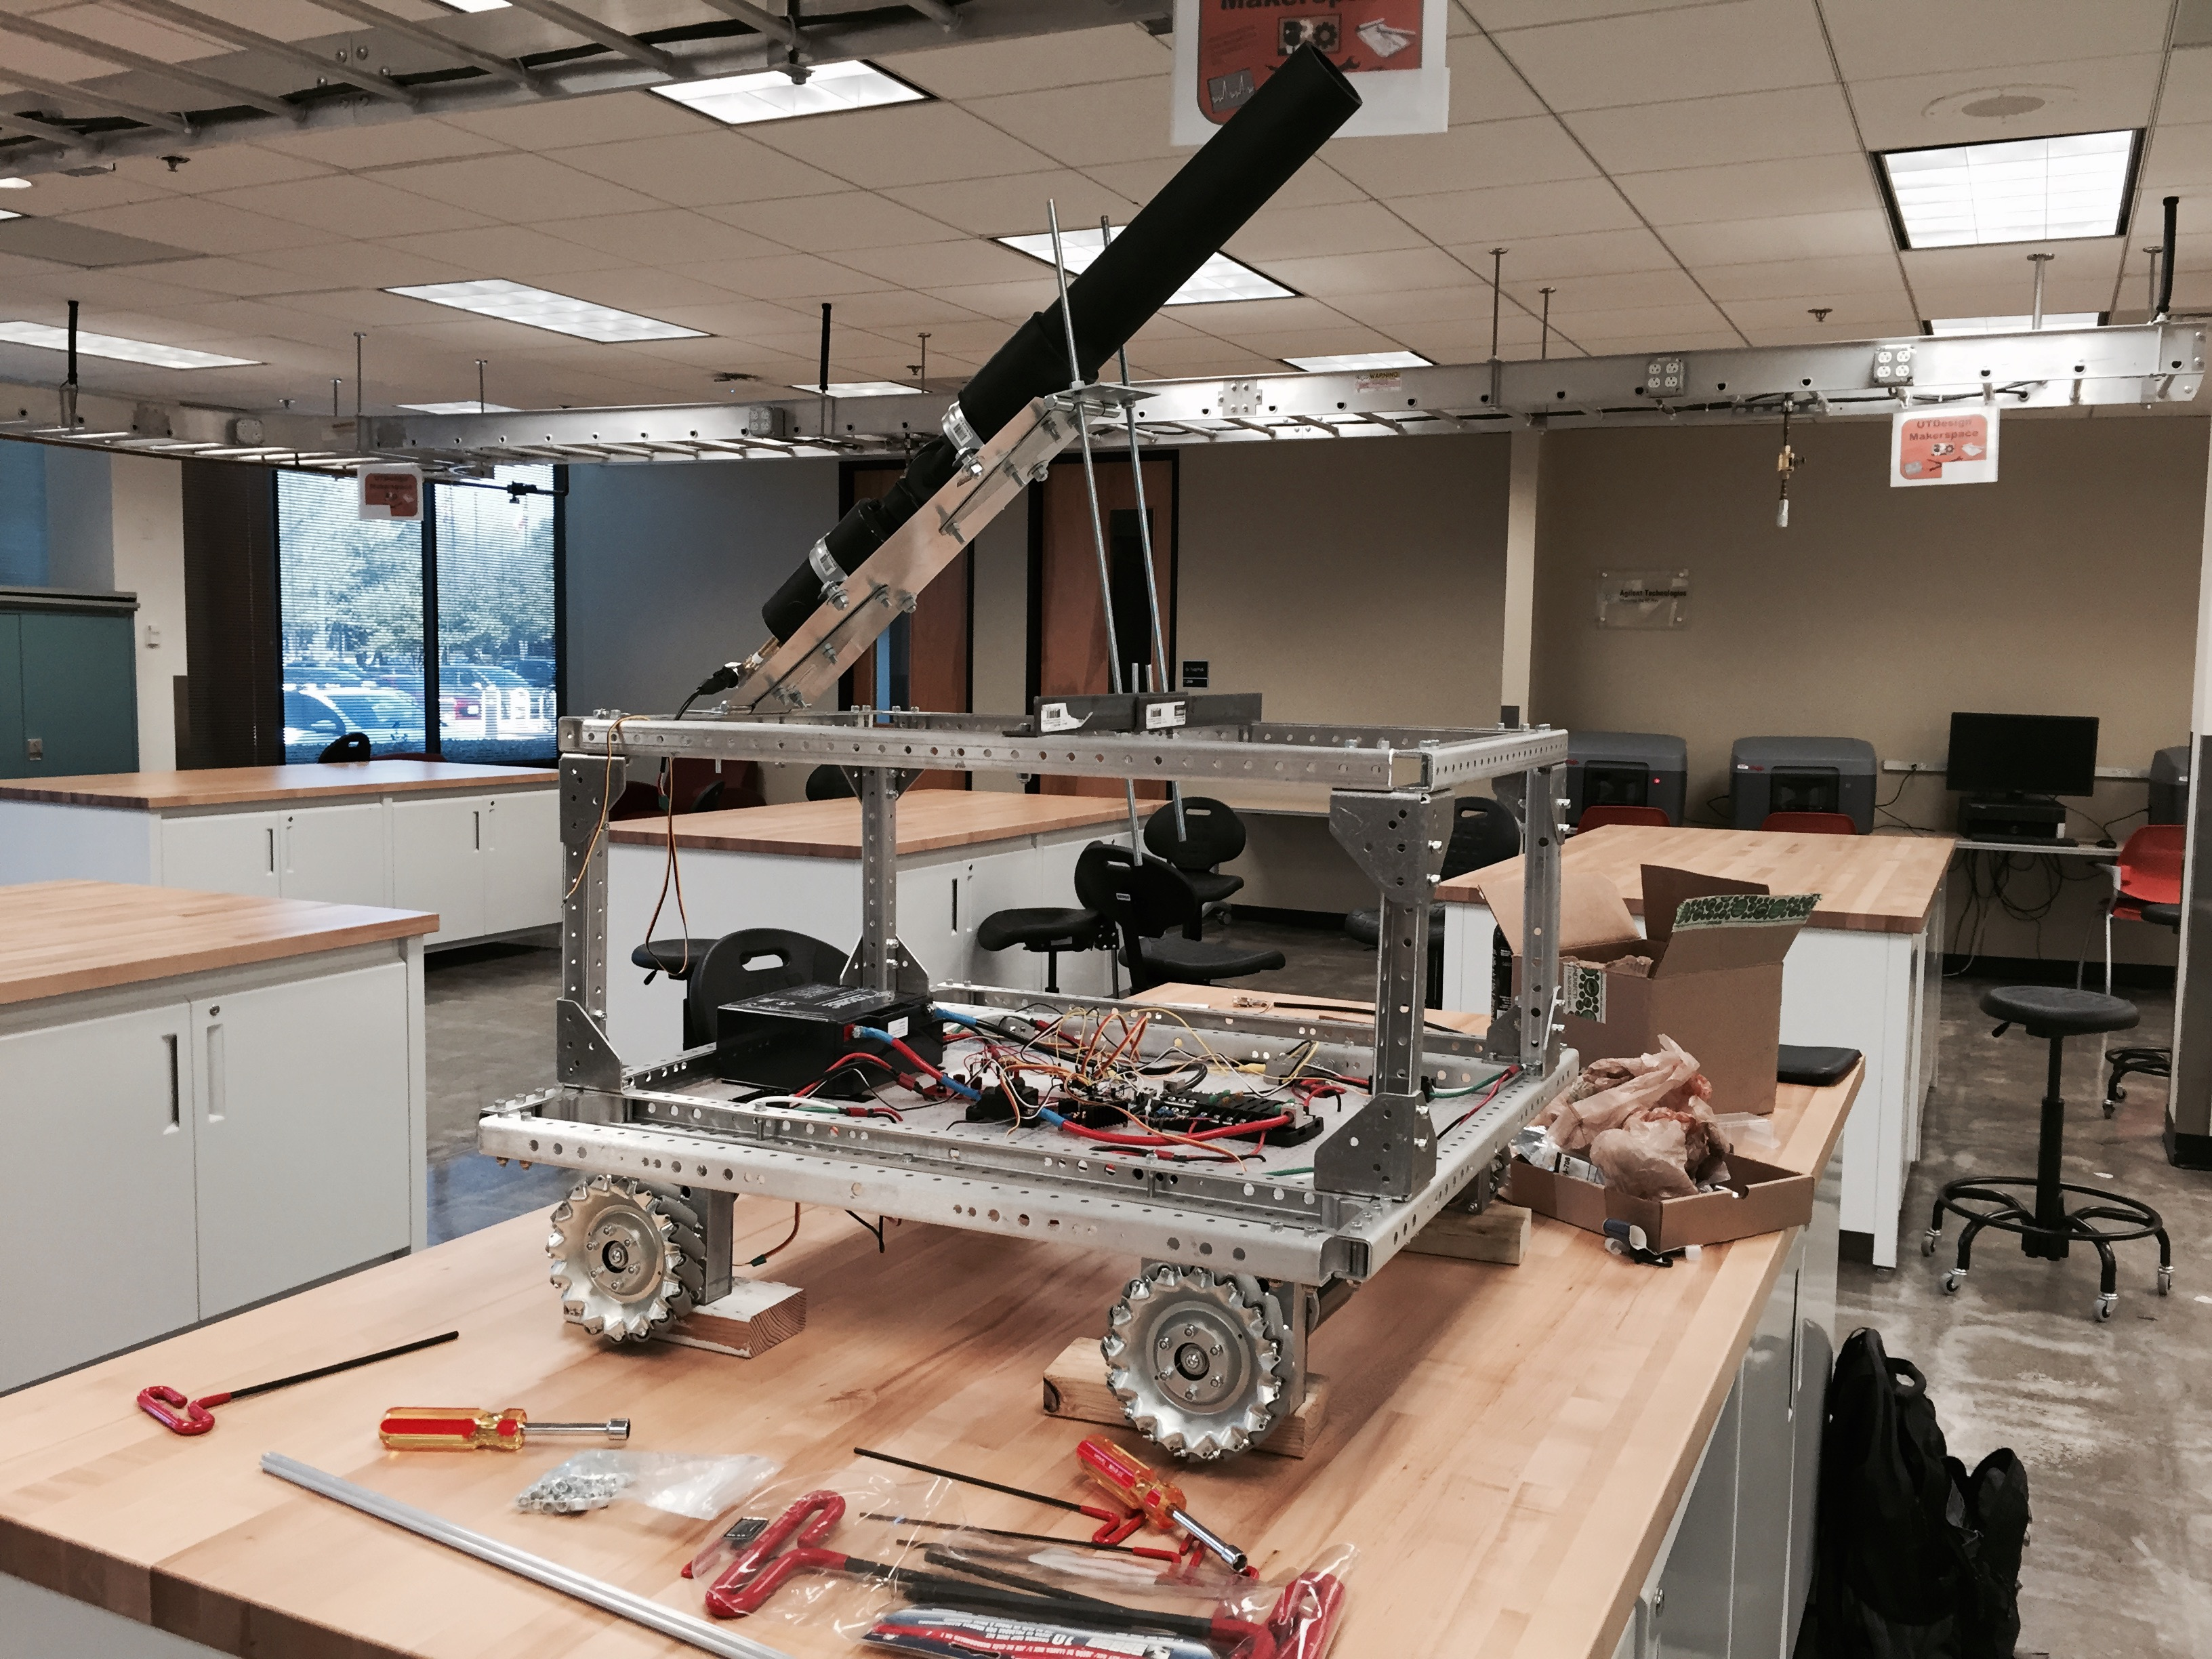
\includegraphics[width=14cm]{./pics/chassis/robot.jpg}
    \caption{The \botname at Synergy Park North (SPN)}
\end{figure}

\pagebreak
\tableofcontents
\pagebreak

\chapter{System Design Overview}
The system design for the \botname can be separated into three components.
These components are in order: Mechanical, Electrical, and Software. In the
following sections, the conceptual design of the robot will be made clear. In
the next few chapters, the physical components and their specifications will be
presented.

\section{Mechanical Design Overview}
The mechanical design requirements are as follows:

\begin{enumerate}
    \item Move from one point to another on a flat surface.
    \item Launch soft projectiles at a controllable range of distances from
        itself. This range would preferably be from around 10 feet to 100 feet.
\end{enumerate}

As one can imagine, there are many ways to satisfy these requirements that
don't require ingenuity. For simplicity, the robot was conceptualized to
have 4-wheel drive, a rectangular prism chassis, and a launching mechanism
mounted atop this chassis.\\

A solution for the 4-wheel drive flat chassis was already commercially
available at AndyMark
\subsection{Velocity Kinematics}
\label{sec:ar9331_vel_kin}

In order to command a desired robot velocity,
\begin{math}
    v= [ v_x \quad v_y \quad \omega_z ]^T
\end{math}
, we calculate the wheel velocities as shown in Equations
\ref{eq:rw_to_v}-\ref{eq:v_wheel_4}, according to Figure
\ref{fig:robot_top_view}.

\begin{figure}[h!]
  \centering
  \includestandalone[width=0.5\textwidth]{./tikz-figures/kinematics}
  \caption{Top View of Robot}
  \label{fig:robot_top_view}
\end{figure}

\begin{equation}
  v_{wheel}=r_{wheel}\omega_{wheel}
  \label{eq:rw_to_v}
\end{equation}
\begin{equation}
  v_{wheel\,0}=v_x-v_y-(l_1+l_2)\omega_z
  \label{eq:v_wheel_1}
\end{equation}
\begin{equation}
  v_{wheel\,1}=v_x+v_y+(l_1+l_2)\omega_z
  \label{eq:v_wheel_2}
\end{equation}
\begin{equation}
  v_{wheel\,2}=v_x-v_y+(l_1+l_2)\omega_z
  \label{eq:v_wheel_3}
\end{equation}
\begin{equation}
  v_{wheel\,3}=v_x+v_y-(l_1+l_2)\omega_z
  \label{eq:v_wheel_4}
\end{equation}

\begin{table}[h!]
  \centering
  \begin{tabular}{| c | c |}
    \hline
    \textbf{Motor} & \textbf{Position} \\
    \hline
    0 & Forward Left \\
    \hline
    1 & Forward Right \\
    \hline
    2 & Rear Right \\
    \hline
    3 & Rear Left \\
    \hline
  \end{tabular}
  \caption{Motor Numbers}
  \label{tab:motor_nums}
\end{table}

\section{Electrical Design Overview}
\begin{figure}[h!]
  \centering
  \includestandalone[width=0.8\textwidth]{./tikz-figures/electroncs-overview}
  \caption{Electrical System Diagram}
  \label{fig:e_system}
\end{figure}

\section{Software Design Overview}
\begin{figure}[h!]
  \centering
  \includestandalone[width=0.8\textwidth]{./tikz-figures/software-overview}
  \caption{Software System Diagram}
  \label{fig:system_diagram}
\end{figure}

\chapter{Mechanical Components}
\section{Chassis}
\begin{center}
    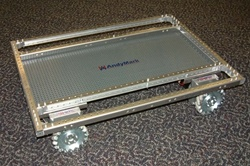
\includegraphics[width=11cm]{pics/chassis/andymark_chassis.jpg}
\end{center}

The Robot's Chassis is the AndyMark C-Chassis with Mecanum Wheel Drive. This
chassis was chosen among others because of its price, modularity, and size.

\subsection{Assembly}
\subsection{References}

\begin{table}[h!]
  \begin{tabular}{| c | c |}
    \hline
    \textbf{AndyMark Frame Assembly} &  http://files.andymark.com/am-0952AssemblyInstructions.pdf\\
    \hline
    \textbf{AndyMark Gearbox Assembly} &  http://files.andymark.com/x2010-toughbox-user-guide.pdf\\
    \hline
  \end{tabular}
  \label{tab:fire_cmd_msg}
\end{table}

\section{T-Shirt Cannon}
\begin{center}
    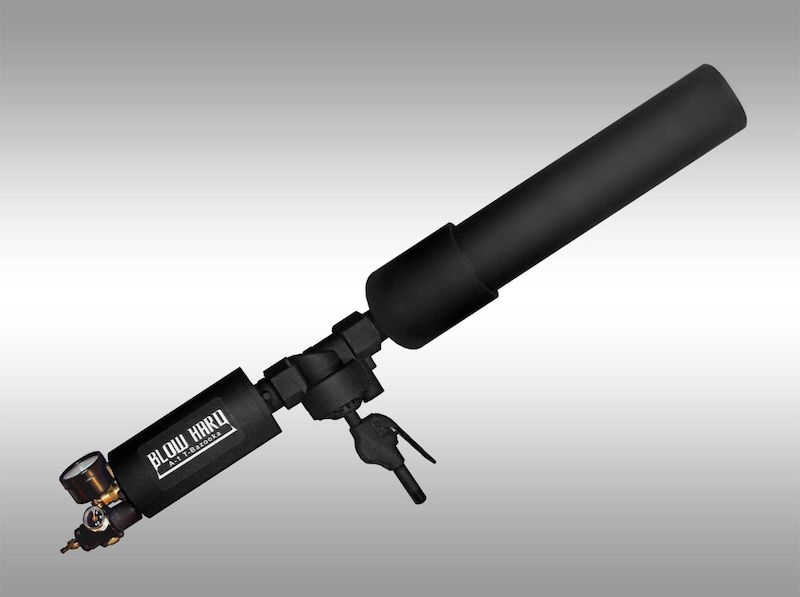
\includegraphics[width=11cm]{pics/cannon/blowhard_cannon.jpg}
\end{center}

\chapter{Electrical Components}

\section{Microcontrollers}
\subsection{AR9331}

\subsection{Serial Communication}
\label{sec:ar9331_serial_com}
The AR9331 and ATMega32U4 communicate via serial. To do this, we open the proper
serial device (\texttt{/dev/ttyATH0}) and use the straightforward
\texttt{write()} command. No further configuration of the serial device is
necessary.

\subsection{ATmega32u4}

\paragraph{Serial Communication}
\label{sec:atmega_serial_com}

Serial communication can occur between the ATmega and AR9331 chips or between
the ATmega chip and a computer connected via USB. In the former case, we read
and write to \texttt{Serial1}, whereas in the latter, we utilize the typical
\texttt{Serial}.

\subsection{Raspberry Pi}

\chapter{Software Components}
\section{Java Application}

\section{Network Protocols}

\subsection{Message Formats}

\paragraph{Computer to Robot}
\label{sec:comp_robot_msg}

\begin{table}[h!]
  \centering
  \begin{tabular}{| l | c | c | c | c | c | c | c | c |}
    \hline
    & 0 & 1 & 2 & 3 & 4 & 5 & 6 & 7 \\
    \hline
    \textbf{Kill Robot} & 0x47 & 0x41 & 0x4e & 0x53 & 0 & & & \\
    \hline
    \textbf{Kill Motors} & 0x47 & 0x41 & 0x4e & 0x53 & 1 & & & \\
    \hline
    \textbf{Command Horn} & 0x47 & 0x41 & 0x4e & 0x53 & 2 & & & \\
    \hline
    \multirow{2}{*}{\textbf{Command Velocity}} & \multirow{2}{*}{0x47} &\multirow{2}{*}{0x41} & \multirow{2}{*}{0x4e} &   \multirow{2}{*}{0x53} & \multirow{2}{*}{3} & v$_x$ & v$_y$ & $\omega_z$ \\
    & & & & & & -128 to 127 & -128 to 127 & -128 to 127 \\
    \hline
    \textbf{Query Motors} & 0x47 & 0x41 & 0x4e & 0x53 & 4 & & & \\
    \hline
    \textbf{Fire Cannon} & 0x47 & 0x41 & 0x4e & 0x53 & 5 & & & \\
    \hline
    \multirow{2}{*}{\textbf{Command Motor}} & \multirow{2}{*}{0x47} &\multirow{2}{*}{0x41} & \multirow{2}{*}{0x4e} &   \multirow{2}{*}{0x53} & \multirow{2}{*}{6} & Motor & Value & \\
    & & & & & & 0 to 3 & -128 to 127 & \\
    \hline
    \multirow{2}{*}{\specialcell{\textbf{Command and}\\\textbf{Control Velocity}}} & \multirow{2}{*}{0x47} &\multirow{2}{*}{0x41} & \multirow{2}{*}{0x4e} &   \multirow{2}{*}{0x53} & \multirow{2}{*}{7} & v$_x$ & v$_y$ & $\omega_z$ \\
    & & & & & & -128 to 127 & -128 to 127 & -128 to 127 \\
    \hline
    \textbf{Increase Pressure} & 0x47 & 0x41 & 0x4e & 0x53 & 8 & & & \\
    \hline
    \textbf{Query Pressure} & 0x47 & 0x41 & 0x4e & 0x53 & 9 & & & \\
    \hline
    \textbf{AVR Debug} & 0x47 & 0x41 & 0x4e & 0x53 & 10 & & & \\
    \hline
    \textbf{Atheros Debug} & 0x47 & 0x41 & 0x4e & 0x53 & 11 & & & \\
    \hline
  \end{tabular}
  \caption{Computer-to-Robot Message Specifications}
  \label{tab:comptorobotmsgspecs}
\end{table}

\paragraph{Robot to Computer}

\paragraph{AR9331 to ATmega32u4}
\label{sec:ath_mega_msg}

\xxx{Query commands will start at 101, but we have yet to come up with the types that we need}

\begin{table}[h!]
  \centering
  \begin{tabular}{| c | c | c|}
    \hline
    \textbf{Byte} & 0-3 & 4 \\
    \hline
    \textbf{Description} & \specialcell{Magic\\Bytes} & \specialcell{Command\\Type} \\
    \hline
    \textbf{Value} & 0x47414e53 & 0 \\
    \hline
  \end{tabular}
  \caption{Kill Command Message Format}
  \label{tab:ath_kill_cmd_msg}
\end{table}

\begin{table}[h!]
  \centering
  \begin{tabular}{| c | c | c|}
    \hline
    \textbf{Byte} & 0-3 & 4 \\
    \hline
    \textbf{Description} & \specialcell{Magic\\Bytes} & \specialcell{Command\\Type} \\
    \hline
    \textbf{Value} & 0x47414e53 & 1 \\
    \hline
  \end{tabular}
  \caption{Keep Alive Command Message Format}
  \label{tab:ath_keep_alive_cmd_msg}
\end{table}

\begin{table}[h!]
  \centering
  \begin{tabular}{| c | c | c | c | c |}
    \hline
    \textbf{Byte} & 0-3 & 4 & 5 & 6 \\
    \hline
    \textbf{Description} & \specialcell{Magic\\Bytes} & \specialcell{Command\\Type} & \specialcell{Motor\\Number} & Value \\
    \hline
    \textbf{Value} & 0x47414e53 & 2 & 0-3 & -128 to 127 \\
    \hline
  \end{tabular}
  \caption{Individual Motor Command Message Format}
  \label{tab:ath_ind_motor_cmd_msg}
\end{table}

\begin{table}[h!]
  \centering
  \begin{tabular}{| c | c | c | c | c | c | c |}
    \hline
    \textbf{Byte} & 0-3 & 4 & 5 & 6 & 7 & 8\\
    \hline
    \textbf{Description} & \specialcell{Magic\\Bytes} & \specialcell{Command\\Type} & \specialcell{Motor 0\\Value} & \specialcell{Motor 1\\Value} & \specialcell{Motor 2\\Value} & \specialcell{Motor 3\\Value} \\
    \hline
    \textbf{Value} & 0x47414e53 & 3 & -128 to 127 & -128 to 127 & -128 to 127 & -128 to 127 \\
    \hline
  \end{tabular}
  \caption{All Motor Command Message Format}
  \label{tab:ath_all_motor_cmd_msg}
\end{table}

\begin{table}[h!]
  \centering
  \begin{tabular}{| c | c | c | c | c |}
    \hline
    \textbf{Byte} & 0-3 & 4 & 5 \\
    \hline
    \textbf{Description} & \specialcell{Magic\\Bytes} & \specialcell{Command\\Type} & \specialcell{Motor\\Number} \\
    \hline
    \textbf{Value} & 0x47414e53 & 4 & 0-3 \\
    \hline
  \end{tabular}
  \caption{Individual Motor Command for Returning Measured Angular Velocity}
  \label{tab:ath_ind_motor_cmd_msg}
\end{table}

\begin{table}[h!]
  \centering
  \begin{tabular}{| c | c | c |}
    \hline
    \textbf{Byte} & 0-3 & 4 \\
    \hline
    \textbf{Description} & \specialcell{Magic\\Bytes} & \specialcell{Command\\Type} \\
    \hline
    \textbf{Value} & 0x47414e53 & 5 \\
    \hline
  \end{tabular}
  \caption{Fire Command Message Format}
  \label{tab:comp_fire_cmd_msg}
\end{table}

\begin{table}[h!]
  \centering
  \begin{tabular}{| c | c | c | c | c |}
    \hline
    \textbf{Byte} & 0-3 & 4 & 5 & 6 \\
    \hline
    \textbf{Description} & \specialcell{Magic\\Bytes} & \specialcell{Command\\Type} & \specialcell{Motor\\Number} & Value \\
    \hline
    \textbf{Value} & 0x47414e53 & 6 & 0-3 & -128 to 127 \\
    \hline
  \end{tabular}
  \caption{Individual Motor Velocity Command Message Format}
  \label{tab:ath_ind_motor_cmd_msg}
\end{table}

\begin{table}[h!]
  \centering
  \begin{tabular}{| c | c | c | c | c | c | c |}
    \hline
    \textbf{Byte} & 0-3 & 4 & 5 & 6 & 7 & 8\\
    \hline
    \textbf{Description} & \specialcell{Magic\\Bytes} & \specialcell{Command\\Type} & \specialcell{Motor 0\\Value} & \specialcell{Motor 1\\Value} & \specialcell{Motor 2\\Value} & \specialcell{Motor 3\\Value} \\
    \hline
    \textbf{Value} & 0x47414e53 & 7 & -128 to 127 & -128 to 127 & -128 to 127 & -128 to 127 \\
    \hline
  \end{tabular}
  \caption{All Motor Velocity Command Message Format}
  \label{tab:ath_all_motor_cmd_msg}
\end{table}

\begin{table}[h!]
  \centering
  \begin{tabular}{| c | c | c | c | c | c |}
    \hline
    \textbf{Byte} & 0-3 & 4 & 5-6 \\
    \hline
    \textbf{Description} & \specialcell{Magic\\Bytes} & \specialcell{Command\\Type} & \specialcell{Pressure\\(Big Endian)} \\
    \hline
    \textbf{Value} & 0x47414e53 & 8 & 0-1023 \\
    \hline
  \end{tabular}
  \caption{Set Pressure Regulation Command}
  \label{tab:ath_ind_motor_cmd_msg}
\end{table}

\paragraph{ATmega32u4 to AR9331}
\label{sec:mega_ath_msg}

\chapter{Future Work}

This chapter suggests future improvements to the robot that were not within the
reach of the project's original scope. The suggestions are presented in order
of precedence.

\section{Network Improvements}
Under our current implementation, the user connects a laptop to a mobile ad hoc
network to which the Raspberry Pi and Arduino Yun are already connected. While
our configuration does work, its performance is suboptimal and could be
improved. The largest problem plaguing the network is that video streaming is
very bandwidth-intensive. This causes the video stream to have large amounts of
latency at times, and sometimes this latency seeks into the controls of the
robot as well. Video streaming will always be bandwidth-intensive, and video
streaming through a mobile ad hoc network will always be troublesome. One
improvement that could be made, though, is to switch the transport protocol of
the video stream from TCP to UDP. TCP has more overhead than UDP, which can
cause large amounts of latency, particularly as a link deteriorates. Even if the
video streaming performance is not optimal, changes could be made so that the
video streaming does not affect the robot controls as drastically. Namely, we
could introduce Quality of Service considerations into the network devices such
that the control packets are prioritized over the video stream packets.

\section{Atheros and AVR communication issues}
This issue is further detailed in issue 3 of our \github.  From the user
standpoint, the issue is that the user is not currently receiving any feedback
from the robot. Ideally, the robot would send back the speed of each of its
wheels as well as the pressure in the cannon's tank upon user request.

\section{Automated Cannon Reloading}
One of the most desirable additions to the robot would be a mechanism that
allows automated reloading of the cannon. When we demonstrate the cannon to the
public, this is one of the most requested features. It would be very cool to
have the robot be able to fire a volley of t-shirts before having to return to
the user for reloading. Though this is highly desirable, it is also very
difficult. We discussed a few possibilities for this, including a conveyor belt
system and a gattling gun design. Both of these would likely require a team of
mechanical engineers to implement effectively.

\section{Tilting Cannon Mount}
Another further refinement regarding the cannon is a mechanism to be able to
tilt the cannon. Currently, the cannon is fixed at a 45-degree angle. This does
work sufficiently well for our application, since we can modulate the range of
the shot through changes in the pressure in the cannon's tank. However, it would
be cool for the user to be able to tilt the cannon up and down on command. This
could be accomplished by hinging the back of the robot and using a linear
actuator to tilt the front up and down.

\section{Encoders}
Encoders are attached to the shaft of each of the robot's wheels, however the
Yun is not currently connected to any of them. If one were to hook up the yun
to the encoders via the prototyping board that the yun currently plugs into,
then it is possible for the yun to calculate the rotational speed of each of
the wheels. The code for this is already implemented as a small encoder library
available on the \github.

\section{Remote Teloperation}
Though this falls outside the bounds of the intended application for this robot,
remote teleoperation would be a very interesting application. The user could
utilize the video stream coming from the robot to monitor the robot's progress
and send commands with the controller. We attempted to do this by connecting the
robot to the school's network. However, due to the restrictions of the network's
firewall, it is not possible to connect devices together on that particular
network. A more robust solution would be to set up an internet-connected server
dedicated to this purpose. Both the robot and the user would then just connect
to the internet and access the server. The server would be able to relay
commands from the user to the robot and send the video stream back to the user.

\section{Computer Vision}
Our original motivation for putting the camera on the robot was to provide a
sensor for some computer vision applications. We ended up not really pursuing
this due to time constraints, but there are many interesting possibilities. One
option would be to implement a ``targeting'' mechanism by which the robot could
autonomously aim and fire at targets based on their color. Another option would
be to implement visual servoing as a closed-loop control mechanism for the
robot.

\section{Cannon Failsafe}
One of our primary concerns throughout the project was ensuring the safety of
the user and the public. Because we are firing projectiles at a high rate of
speed, there is the potential for injury. The most concerning situation would be
if a person was very close to the cannon and it was triggered. Currently, we are
relying mainly on the judgment of the operator to avoid such incidents. However,
safety measures should probably be implemented to make the cannon more failsafe
in this regard. Specifically, we should have a mechanism that disables the
cannon from firing if any object is within a certain range of it. The best idea
that we had for implementing this was with a laser rangefinder that reported the
distance to the closest object. If the sensor indicates that an object is in the
path of the cannon, the MCU disables the cannon's triggering mechanism.

\section{Recharging Circuit}
Currently, in order to recharge the robot's battery, one must remove the
battery from the robot, which requires unscrewing two bolts. It would be ideal
if a charging circuit were included on the robot so that one doesn't have to
remove this battery. We envision plugging the robot into a wall socket and
letting it charge overnight. Google `Battery University' for more info about
charging lead acid batteries. You can also google `Lead Acid Battery Charger'
for examples of these types of chargers.

\section{Turbo Mode}
The robot has a top speed of around 6 mph in the forward direction and 4 mph
laterally. However, we have limited the speed of the robot in software so that
it can only move at approximately half of its maximum speed. We did this for
several reasons, including safety and usability. However, it would be good for
the full potential of this robot to be accessible to the user if desired. This
could be implemented in the form of a ``Turbo Mode'' in which the user holds
down a button on the controller to get a speed boost. In addition to software
changes that must occur for this to be possible, we also need to add larger
charging capacitors in order to counteract the large current draws that are
demanded during quick accelerations.

\section{Mobile Application}
As we have driven the robot around campus, we have realized that it is actually
quite burdensome to only be able to control it from a desktop application. From
a usability perspective, it would be much nicer to have the option of using a
mobile application, particularly if the user is also mobile. To avoid the
trouble of creating separate applications to support the various mobile
platforms (iOS, Android, Windows), it may be preferable to create a
browser-based application.

\chapter{Robot Operation}

\section{Running the video stream from outside the app}
nc 192.168.1.1 5001 | mplayer -fps 60 -cache 1024 -

\chapter{Troubleshooting}

\section{Mechanical Issues}
\subsection{Chassis}
\subsection{T-Shirt Cannon}

\begin{center}
    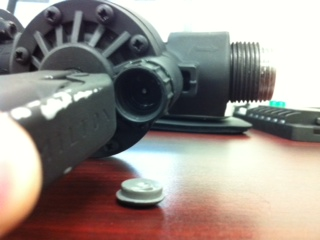
\includegraphics[width=11cm]{pics/cannon/broken_release_valve.jpg}
\end{center}

\section{Electrical Issues}

\section{Software Issues}
\subsection{Site to install xbox controller drivers}
OSX: http://tattiebogle.net/index.php/ProjectRoot/Xbox360Controller/OsxDriver


\end{document}
